\autobookmark
\begin{frame}[t]{Adaptive number of rays to counter high MSE values}
  \begin{columns}[T]
    \begin{column}{.5\textwidth}
      \hfill
      \myonly{1}{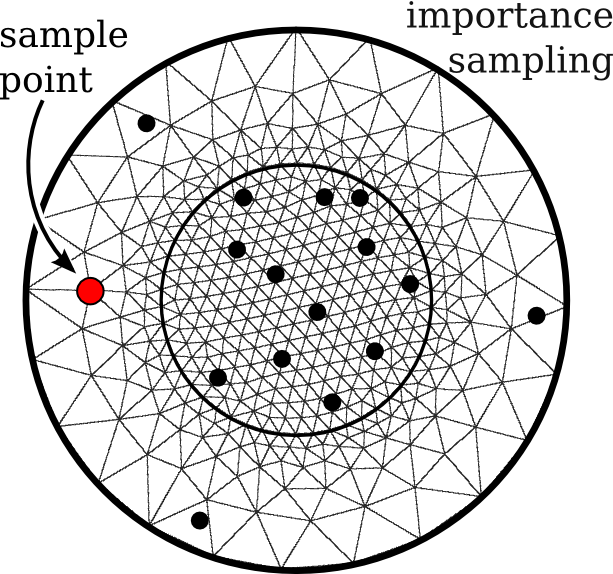
\includegraphics[width=.7\textwidth]{graphics/ray_distributions3.png}}
      \myonly{2}{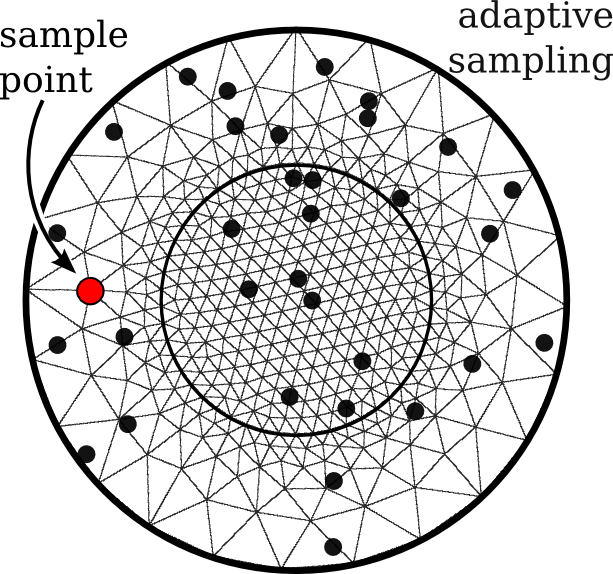
\includegraphics[width=.7\textwidth]{graphics/ray_distributions4.png}}\\[1ex]
      \hfill
      \myonly{1}{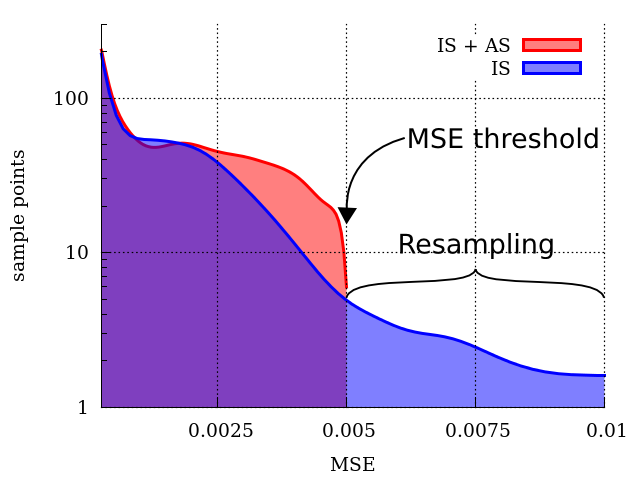
\includegraphics[width=.7\textwidth]{graphics/mse_adaptive.png}}
      \myonly{2}{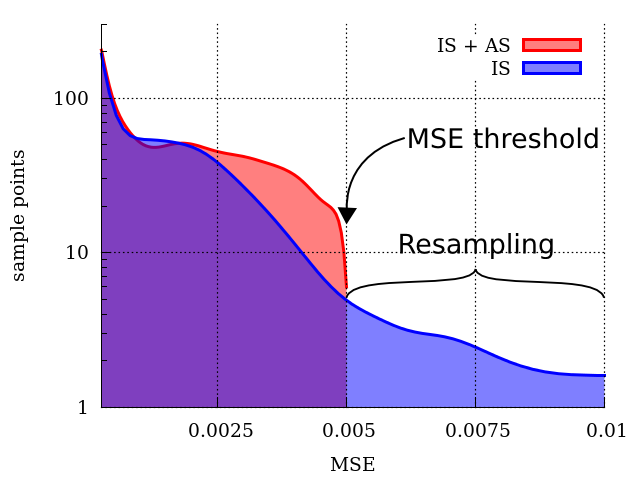
\includegraphics[width=.7\textwidth]{graphics/mse_adaptive.png}}
    \end{column}
    \begin{column}{.5\textwidth}
      \begin{itemize}
        \item If the MSE is too high, repeat processing for this sample point with more rays
        \item This adaptive sampling can limit the maximal MSE to a fixed threshold
      \end{itemize}
    \end{column}
  \end{columns}
\end{frame}

%\begin{frame}{Predefined colours}
%  The template defines a set of colours according to the CD guidelines:\par
%  \begin{itemize}
%      \begin{minipage}[t]{0.5\linewidth}
%      \item \textcolor{hzdr-blue}{Helmholtz Blue}    
%      \item \textcolor{hzdr-orange}{Rossendorf Orange}  
%      \item \textcolor{hzdr-darkblue}{Helmholtz Dark Blue}
%      \item \textcolor{hzdr-gray1}{Gray1}   
%      \item \textcolor{hzdr-gray2}{Gray2}   
%      \item \textcolor{hzdr-gray3}{Gray3}   
%      \item \textcolor{hzdr-struct}{Structure of Matter}  
%      \end{minipage}%
%      \begin{minipage}[t]{0.5\linewidth}
%      \item \textcolor{hzdr-health}{Health}  
%      \item \textcolor{hzdr-energy}{Energy}  
%      \item \textcolor{hzdr-earth}{Earth and Environment}   
%      \item \textcolor{hzdr-keytec}{Key Technologies}  
%      \item \textcolor{hzdr-aero}{Aeronautics, Space and Transport}
%      \end{minipage}
%  \end{itemize}
%\end{frame}

